\section{热核}
\label{sec:heat-kernel}

棒无限长时没有端点来挑选模式，频率不再是离散的$k\pi$，而是连成一片。此时局部的一点热量怎样影响后来的场？我们考虑全空间的问题
\begin{equation}
 \partial_tu=\Delta u,\quad \bm{x}\in\mathbb{R}^{d},\ t>0;\qquad u(\bm{x},0)=u_0(\bm{x}) .
 \label{eq:heat-cauchy}
\end{equation}
先用Fourier变换形式地求出公式，再撇开形式推导，直接检验公式在什么条件下给出解、在什么意义下取回初值。

\subsection{核的构造}
\label{sec:heat-kernel-construction}

\paragraph{每个频率一个标量方程}
沿用卷四的约定，Fourier变换写成
\[
 \widehat{u}(\bm{\xi})=\int u(\bm{x})\mathrm{e}^{-2\pi\mathrm{i}\bm{x}\cdot\bm{\xi}}\,\mathrm{d}\bm{x} .
\]
这时对$x_j$求导对应乘以$2\pi\mathrm{i}\xi_j$，Laplace算子对应乘以$-4\pi^2\lvert\bm{\xi}\rvert^2$，这些运算规则都在上一节所引的卷四一章中建立。

设$u$足够好，对式~\eqref{eq:heat-cauchy}关于$\bm{x}$作变换。偏微分方程对每个固定的$\bm{\xi}$变成一个标量常微分方程：
\[
 \partial_t\widehat{u}(\bm{\xi},t)=-4\pi^2\lvert\bm{\xi}\rvert^2\,\widehat{u}(\bm{\xi},t) .
\]
这与上一节的$a'=-\lambda a$完全相同，只是$\lambda$换成了连续变化的$4\pi^2\lvert\bm{\xi}\rvert^2$。解出来是
\begin{equation}
 \widehat{u}(\bm{\xi},t)=\mathrm{e}^{-4\pi^2\lvert\bm{\xi}\rvert^2t}\,\widehat{u}_0(\bm{\xi}) .
 \label{eq:heat-fourier-solution}
\end{equation}
两种模式的对应是精确的：$\sin(k\pi x)=\sin(2\pi(k/2)x)$的频率是$\xi=k/2$，代入$4\pi^2\xi^2$恰好得到$k^2\pi^2$。

\paragraph{乘法还原为卷积}
频域的乘积对应空间的卷积，所以只需找到一个函数，它的变换是$\mathrm{e}^{-4\pi^2\lvert\bm{\xi}\rvert^2t}$。卷四已经算过：$\mathrm{e}^{-\pi\lvert\bm{x}\rvert^2}$的变换是它自身；又把函数$g(\bm{x})$换成$s^{-d}g(\bm{x}/s)$，变换从$\widehat{g}(\bm{\xi})$变成$\widehat{g}(s\bm{\xi})$。

要让指数对上，需要$\pi s^2=4\pi^2t$，即$s=\sqrt{4\pi t}$，这样就得到下面的函数。

\begin{definition}[热核]
\label{def:heat-kernel}
$\mathbb{R}^{d}$上的\term{热核}（heat kernel）是
\begin{equation}
 G(\bm{x},t)=\frac{1}{(4\pi t)^{d/2}}\exp\Bigl(-\frac{\lvert\bm{x}\rvert^2}{4t}\Bigr),\qquad \bm{x}\in\mathbb{R}^{d},\ t>0 .
 \label{eq:heat-kernel}
\end{equation}
对初值$u_0$，定义\term{卷积表示}（convolution representation）
\begin{equation}
 u(\bm{x},t)=\int_{\mathbb{R}^{d}}G(\bm{x}-\bm{y},t)\,u_0(\bm{y})\,\mathrm{d}\bm{y} .
 \label{eq:heat-convolution}
\end{equation}
\end{definition}

到这里的推导要求$u$有变换、能逐点解常微分方程、乘积能还原，都是形式的。下面的做法不再依赖它们，而是直接研究式~\eqref{eq:heat-kernel}和式~\eqref{eq:heat-convolution}。

\begin{theorem}[热核的基本性质]
\label{thm:heat-kernel-properties}
对$t>0$，式~\eqref{eq:heat-kernel}的$G$满足：
\begin{enumerate}
 \item $G>0$，并且$G(\cdot,t)$在$\mathbb{R}^{d}$上的积分等于$1$；
 \item 满足尺度关系
 \begin{equation}
  G(\bm{x},t)=t^{-d/2}G(\bm{x}/\sqrt{t},1) ;
  \label{eq:heat-kernel-scaling}
 \end{equation}
 \item 每个坐标的二阶矩等于$2t$；
 \item 在$\mathbb{R}^{d}\times(0,\infty)$上$\partial_tG=\Delta G$。
\end{enumerate}
\end{theorem}

\begin{proof}
正性由公式可见。积分按坐标分解成$d$个一维积分的乘积。一维情形代换$x=2\sqrt{t}\,z$，
\[
 \int_{\mathbb{R}}\frac{1}{\sqrt{4\pi t}}\mathrm{e}^{-x^2/(4t)}\,\mathrm{d}x=\frac{1}{\sqrt\pi}\int_{\mathbb{R}}\mathrm{e}^{-z^2}\,\mathrm{d}z=1 .
\]
尺度关系由公式直接代入得到。二阶矩中其余坐标积分为$1$，剩下的一维积分用同一代换，再用$\int z^2\mathrm{e}^{-z^2}\,\mathrm{d}z=\sqrt\pi/2$，得到
\[
 \int_{\mathbb{R}}x^2G(x,t)\,\mathrm{d}x=\frac{4t}{\sqrt\pi}\int_{\mathbb{R}}z^2\mathrm{e}^{-z^2}\,\mathrm{d}z=2t .
\]

最后计算导数。令$r=\lvert\bm{x}\rvert$，对$t$求导得到
\[
 \partial_tG=\Bigl(-\frac{d}{2t}+\frac{r^2}{4t^2}\Bigr)G .
\]
对$x_i$求一次导数得$\partial_iG=-\tfrac{x_i}{2t}G$，再求一次并对$i$求和，
\[
 \Delta G=\sum_{i}\Bigl(-\frac{1}{2t}+\frac{x_i^2}{4t^2}\Bigr)G=\Bigl(-\frac{d}{2t}+\frac{r^2}{4t^2}\Bigr)G .
\]
两式相等。
\end{proof}

四条性质各有含义。正性和积分为$1$说卷积是一种加权平均，总热量不变。尺度关系说时间不产生新形状，只把同一个钟形按$\sqrt{t}$拉宽、按$t^{-d/2}$压低。二阶矩说方差随时间线性增长，所以宽度是$\sqrt{2t}$。

具体地，一维时$t=0.01,0.04,0.16$的峰值是$2.82,\,1.41,\,0.705$，标准差是$0.141,\,0.283,\,0.566$：时间变为四倍，宽度加倍，峰值减半，图~\ref{fig:heat-kernel-scaling}。这就是初边值问题里“棒长加倍、时间四倍”的另一面。

\begin{BookInlineFigure}
  \centering
  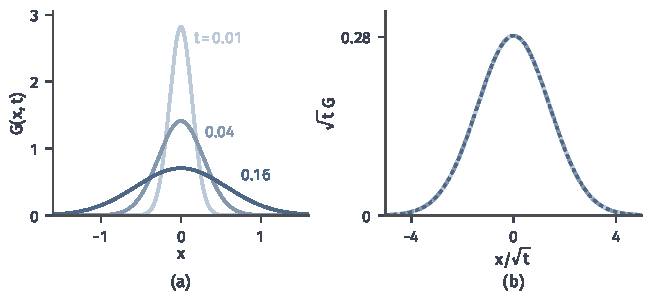
\includegraphics[width=112mm]{figures/06-differential-equations/02-partial-differential-equations/matplotlib/heat-kernel-scaling/figure.pdf}
  \caption{一维热核。(a)$t=0.01,0.04,0.16$时的$G(x,t)$（蓝色由浅到深）。(b)改用尺度化坐标后的$\sqrt{t}\,G$与$x/\sqrt{t}$，三个时刻（实线、虚线、点线）重合到同一条曲线。}
  \label{fig:heat-kernel-scaling}
\end{BookInlineFigure}

\paragraph{卷积是加权平均}
式~\eqref{eq:heat-convolution}的读法是：时刻$t$在$\bm{x}$处的温度，是初值以$\bm{x}$为中心、宽度约$\sqrt{2t}$的Gauss加权平均。也可以反过来读：$\bm{y}$处的一点初始热量$u_0(\bm{y})\,\mathrm{d}\bm{y}$，到时刻$t$散成以$\bm{y}$为中心的钟形，所有钟形叠加成解。

取方框$u_0=\mathbb{I}_{[-1/2,1/2]}$为例。引入误差函数
\[
 \operatorname{erf}(z)=\frac{2}{\sqrt\pi}\int_0^z\mathrm{e}^{-s^2}\,\mathrm{d}s .
\]
一维积分经代换$z=(x-y)/(2\sqrt{t})$化为
\begin{equation}
 u(x,t)=\frac12\Bigl(\operatorname{erf}\frac{x+1/2}{2\sqrt{t}}-\operatorname{erf}\frac{x-1/2}{2\sqrt{t}}\Bigr) .
 \label{eq:heat-box-solution}
\end{equation}

图~\ref{fig:heat-convolution-weights}取$x=0.7$，$t=0.04$。紫色钟形在方框内的部分（蓝色浅底）的面积就是这一点的温度，代入式~\eqref{eq:heat-box-solution}得$0.240$。这一点在方框外，初值为零，可是加权平均已经够到了方框。

\begin{BookInlineFigure}
  \centering
  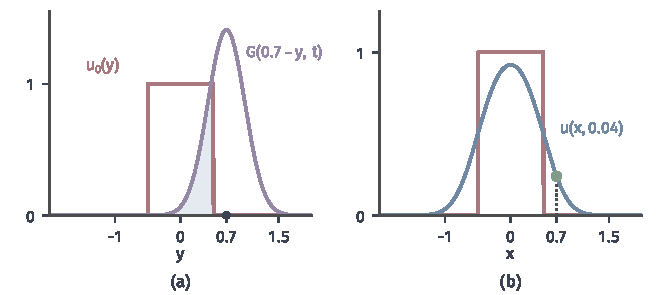
\includegraphics[width=112mm]{figures/06-differential-equations/02-partial-differential-equations/matplotlib/heat-convolution-weights/figure.pdf}
  \caption{卷积作为加权平均。(a)方框初值（红）与以$x=0.7$为中心、$t=0.04$的权重$G(0.7-y,t)$（紫），蓝色浅底的面积等于$u(0.7,0.04)$。(b)解$u(\cdot,0.04)$（蓝），绿点是$x=0.7$处的值$0.240$。}
  \label{fig:heat-convolution-weights}
\end{BookInlineFigure}

\paragraph{传播范围}
热核处处为正，于是只要$u_0\geq0$不恒为零，对任意小的$t>0$，$u$在每一点都严格为正。扰动瞬间到达无穷远，这一性质称为\term{无穷传播速度}（infinite speed of propagation），它与下一章波动方程的有限速度截然不同。

但“到达”的量极小。由式~\eqref{eq:heat-box-solution}，$t=0.01$时距离方框中心$2$的地方温度只有约$1.4\times10^{-26}$，$t=0.1$时距离$3$的地方约$1.1\times10^{-8}$。图~\ref{fig:heat-tails}(a)中尾部在对数坐标下是向下弯的抛物线，这是$\mathrm{e}^{-x^2/(4t)}$的特征。

想知道“热量实际传到哪里”，可以固定一个小的阈值看等值线。图~\ref{fig:heat-tails}(b)是$u=10^{-3}$的位置，它按$\sqrt{t}$前进，早期很快，后来越来越慢，并不是匀速推进的波前。

\begin{BookInlineFigure}
  \centering
  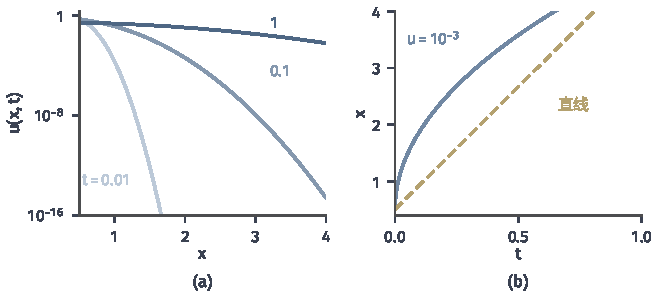
\includegraphics[width=112mm]{figures/06-differential-equations/02-partial-differential-equations/matplotlib/heat-tails/figure.pdf}
  \caption{方框初值的远场。(a)$x>1/2$上的解，纵轴对数，$t=0.01,0.1,1$（蓝色由浅到深）。(b)等值线$u=10^{-3}$的位置（蓝），黄色虚线是连接其起点和终点的直线，匀速前进的前沿应当沿这样的直线。}
  \label{fig:heat-tails}
\end{BookInlineFigure}

这里要说清类比的边界。把热核读成“热量瞬间传到远处”，描述的是这个数学模型。真实的热传递由有限速度的微观运动实现，Fourier定律只是在足够大的尺度上的近似，远处$10^{-26}$量级的温度变化没有物理意义。模型的价值在于$\sqrt{t}$的尺度和被压到极小的尾部，而不在严格的正性上。

\paragraph{频率的衰减}
同一个解也可以在频域读。式~\eqref{eq:heat-fourier-solution}说，频率$\bm{\xi}$的分量乘以$\mathrm{e}^{-4\pi^2\lvert\bm{\xi}\rvert^2t}$。这个因子在$\lvert\bm{\xi}\rvert=1/(2\pi\sqrt{t})$处降到$\mathrm{e}^{-1}$，更高的频率几乎全被抹掉。例如$t=0.01$时$\xi=5$的因子是$\mathrm{e}^{-\pi^2}\approx5\times10^{-5}$。

所以热核是一个低通滤波器，时间越长，通带越窄，图~\ref{fig:heat-fourier-multiplier}。空间和频率的两种读法互为对偶：空间上钟形的宽度按$\sqrt{t}$增长，频率上通带的宽度按$1/\sqrt{t}$收缩。方框的尖角含有缓慢衰减的高频，滤掉之后角就圆了。

\begin{BookInlineFigure}
  \centering
  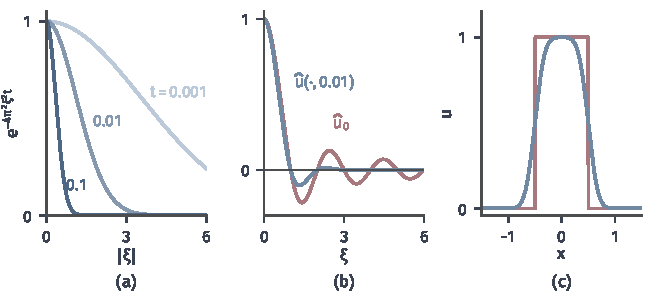
\includegraphics[width=112mm]{figures/06-differential-equations/02-partial-differential-equations/matplotlib/heat-fourier-multiplier/figure.pdf}
  \caption{热传播的频域作用。(a)乘子$\mathrm{e}^{-4\pi^2\xi^2t}$，$t=0.001,0.01,0.1$（蓝色由浅到深）。(b)方框的变换$\widehat{u}_0=\sin(\pi\xi)/(\pi\xi)$（红）与乘上$t=0.01$的乘子后的结果（蓝）。(c)空间中的方框（红）与$t=0.01$的解（蓝）。}
  \label{fig:heat-fourier-multiplier}
\end{BookInlineFigure}

\paragraph{公式何时给出解}
式~\eqref{eq:heat-convolution}的积分未必收敛。$u_0$可以无界，但不能增长得比核衰减得还快。下面的条件恰好刻画这个界线：存在$T>0$，使
\begin{equation}
 \int_{\mathbb{R}^{d}}\lvert u_0(\bm{y})\rvert\,\mathrm{e}^{-\lvert\bm{y}\rvert^2/(4T)}\,\mathrm{d}\bm{y}<\infty .
 \label{eq:heat-integrability}
\end{equation}
有界的可测函数、$L^p$函数（$1\leq p\leq\infty$）都满足它，并且$T$可以取任意正数。

\begin{theorem}[卷积解的可微性]
\label{thm:heat-convolution-smooth}
设$u_0$可测且满足式~\eqref{eq:heat-integrability}。则式~\eqref{eq:heat-convolution}的积分对$\bm{x}\in\mathbb{R}^{d}$、$0<t<T$绝对收敛，$u$在$\mathbb{R}^{d}\times(0,T)$上无穷次可微，且可以在积分号下求导；特别地
\begin{equation}
 \partial_tu=\Delta u,\qquad \bm{x}\in\mathbb{R}^{d},\ 0<t<T .
 \label{eq:heat-convolution-solves}
\end{equation}
\end{theorem}

\begin{proof}
固定紧集$K\subset\mathbb{R}^{d}\times(0,T)$，其上$\lvert\bm{x}\rvert\leq R$，$t_0\leq t\leq t_1<T$。关键是用一个与$(\bm{x},t)$无关的可积函数控制被积函数及其导数。

取$\theta>0$使$(1+\theta)t_1<T$，再取$\sigma\in(0,1)$，使$(1+\theta)t_1/(1-\sigma)\leq T$。由三角不等式和Young不等式，对任意$\bm{x},\bm{y}$，
\[
 \lvert\bm{y}\rvert^2\leq(1+\theta)\lvert\bm{x}-\bm{y}\rvert^2+\bigl(1+\theta^{-1}\bigr)\lvert\bm{x}\rvert^2 .
\]
把它改写成对$\lvert\bm{x}-\bm{y}\rvert^2$的下界，并用$t\leq t_1$，得到
\[
 \frac{(1-\sigma)\lvert\bm{x}-\bm{y}\rvert^2}{4t}\geq\frac{(1-\sigma)\lvert\bm{y}\rvert^2}{4(1+\theta)t_1}-C_1\geq\frac{\lvert\bm{y}\rvert^2}{4T}-C_1 ,
\]
其中常数$C_1$只依赖$R$、$t_0$、$\theta$、$\sigma$。

$G$对$\bm{x}$、$t$的任意阶导数等于$G$乘以一个$\bm{x}$和$1/t$的多项式。在$K$上这个多项式关于$\lvert\bm{x}-\bm{y}\rvert$有多项式增长，而多项式被指数$\mathrm{e}^{-\sigma\lvert\bm{x}-\bm{y}\rvert^2/(4t)}$压住。于是每个导数的绝对值满足
\[
 \bigl\lvert\partial^{\alpha}_{\bm{x}}\partial_t^{n}G(\bm{x}-\bm{y},t)\bigr\rvert\leq C\,\mathrm{e}^{-(1-\sigma)\lvert\bm{x}-\bm{y}\rvert^2/(4t)}\leq C'\,\mathrm{e}^{-\lvert\bm{y}\rvert^2/(4T)} .
\]
乘以$\lvert u_0\rvert$后可积。由控制收敛定理，积分绝对收敛，且可以在积分号下任意次求导。定理~\ref{thm:heat-kernel-properties}的第四条给出式~\eqref{eq:heat-convolution-solves}。
\end{proof}

这个结论里没有要求初值连续，这是扩散的平滑作用的第一次定量出现，后面还要专门研究。条件中的$T$不能随意增大，下面的例子说明它是准确的。

\begin{example}[快速增长的初值]
\label{ex:heat-gaussian-growth}
取$d=1$，$u_0(x)=\mathrm{e}^{ax^2}$，$a>0$。此时式~\eqref{eq:heat-integrability}成立当且仅当$T<1/(4a)$。式~\eqref{eq:heat-convolution}的指数是$y$的二次式，记$p=1/(4t)-a$，当$t<1/(4a)$时$p>0$。把指数写成
\[
 -py^2+\frac{xy}{2t}-\frac{x^2}{4t} .
\]
由Gauss积分
\[
 \int_{\mathbb{R}}\mathrm{e}^{-py^2+by}\,\mathrm{d}y=\sqrt{\frac{\pi}{p}}\,\mathrm{e}^{b^2/(4p)},
\]
取$b=x/(2t)$，振幅因子是$(4\pi t)^{-1/2}\sqrt{\pi/p}$，它等于$(1-4at)^{-1/2}$。指数部分合并后是$ax^2/(1-4at)$，于是
\begin{equation}
 u(x,t)=\frac{1}{\sqrt{1-4at}}\exp\Bigl(\frac{ax^2}{1-4at}\Bigr),\qquad 0\leq t<\frac{1}{4a} .
 \label{eq:heat-gaussian-growth}
\end{equation}
$t\to1/(4a)$时$u(0,t)\to\infty$，解在有限时间爆炸。
\end{example}

图~\ref{fig:heat-growth-limit}取$a=1/2$，由式~\eqref{eq:heat-gaussian-growth}，爆炸时刻是$t=1/2$。这里的爆炸并不违背“热量被抹平”的直觉：无穷远处温度增长得太快，加权平均从远处吸进来的热量越来越多，直到积分发散。

\begin{BookInlineFigure}
  \centering
  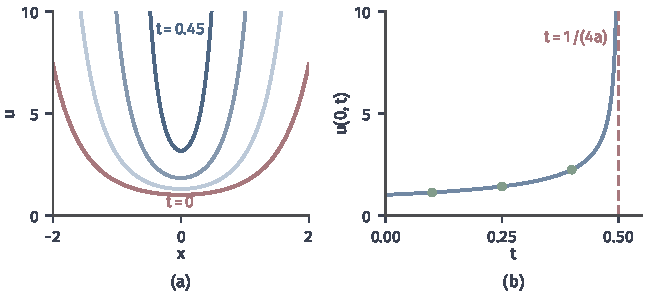
\includegraphics[width=112mm]{figures/06-differential-equations/02-partial-differential-equations/matplotlib/heat-growth-limit/figure.pdf}
  \caption{初值$\mathrm{e}^{x^2/2}$（$a=1/2$）的卷积解。(a)$t=0$（红）与$t=0.2,0.35,0.45$（蓝色由浅到深）。(b)中心温度$u(0,t)=(1-2t)^{-1/2}$（蓝），绿点是直接数值积分的结果，红色虚线是爆炸时刻$t=1/(4a)$。}
  \label{fig:heat-growth-limit}
\end{BookInlineFigure}

\subsection{初值恢复}
\label{sec:heat-recovery}

卷积公式只在$t>0$时有定义，定理~\ref{thm:heat-convolution-smooth}没有提到初值。$t\to0^+$时$u$回到$u_0$吗？答案取决于数据和“回到”的含义。

\paragraph{质量向一点集中}
直观上，$G(\cdot,t)$的总质量始终是$1$，宽度却趋于零，加权平均只看越来越近的邻域，所以应当趋于该点的值。这样的一族函数称为\term{恒同逼近}（approximate identity）。所有证明都用到同一个定量事实：对任意$\delta>0$，由尺度关系~\eqref{eq:heat-kernel-scaling}，
\begin{equation}
 \int_{\lvert\bm{y}\rvert\geq\delta}G(\bm{y},t)\,\mathrm{d}\bm{y}=\int_{\lvert\bm{z}\rvert\geq\delta/\sqrt{t}}G(\bm{z},1)\,\mathrm{d}\bm{z}\ \longrightarrow\ 0,\quad t\to0^+ .
 \label{eq:heat-tail}
\end{equation}
右边是一个可积函数在越来越远的区域上的积分，所以趋于零。图~\ref{fig:heat-approx-identity}显示了$\lvert\bm{y}\rvert\geq\delta$上的尾部质量怎样随$t$变化。

\begin{BookInlineFigure}
  \centering
  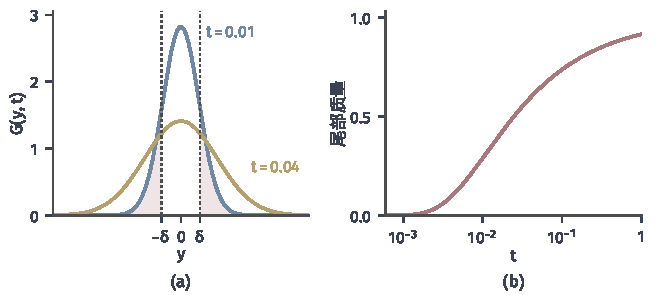
\includegraphics[width=112mm]{figures/06-differential-equations/02-partial-differential-equations/matplotlib/heat-approx-identity/figure.pdf}
  \caption{热核质量的集中。(a)$t=0.01$（蓝）与$t=0.04$（黄）的核，红色浅底是$t=0.01$时$\lvert y\rvert\geq\delta$的尾部，$\delta=0.15$。(b)该尾部质量$\operatorname{erfc}(\delta/(2\sqrt{t}))$随$t$的变化，横轴为对数。}
  \label{fig:heat-approx-identity}
\end{BookInlineFigure}

\paragraph{一致恢复}
记$C_0(\mathbb{R}^{d})$为在无穷远趋于零的连续函数，它们都有界且一致连续，所以只需讨论有界一致连续的函数。一致连续性是这里的关键：同一个$\delta$要对所有的点起作用。

\begin{theorem}[一致范数下的恢复]
\label{thm:heat-uniform-recovery}
设$u_0$在$\mathbb{R}^{d}$上有界且一致连续，特别地可以是$u_0\in C_0(\mathbb{R}^{d})$。则式~\eqref{eq:heat-convolution}给出的$u$满足
\begin{equation}
 \lim_{t\to0^+}\sup_{\bm{x}\in\mathbb{R}^{d}}\lvert u(\bm{x},t)-u_0(\bm{x})\rvert=0 .
 \label{eq:heat-uniform-recovery}
\end{equation}
\end{theorem}

\begin{proof}
因为$G$的积分为$1$，可以把$u_0(\bm{x})$写进积分。再代换$\bm{y}\mapsto\bm{x}-\bm{y}$，
\[
 u(\bm{x},t)-u_0(\bm{x})=\int G(\bm{y},t)\bigl(u_0(\bm{x}-\bm{y})-u_0(\bm{x})\bigr)\,\mathrm{d}\bm{y} .
\]
任取$\varepsilon>0$，由一致连续性取$\delta>0$，使$\lvert\bm{y}\rvert<\delta$时对所有$\bm{x}$都有$\lvert u_0(\bm{x}-\bm{y})-u_0(\bm{x})\rvert<\varepsilon$。

把积分分成$\lvert\bm{y}\rvert<\delta$和$\lvert\bm{y}\rvert\geq\delta$两部分。第一部分不超过$\varepsilon\int G=\varepsilon$。第二部分中被积的差不超过$2\lVert u_0\rVert_\infty$，于是
\[
 \lvert u(\bm{x},t)-u_0(\bm{x})\rvert\leq\varepsilon+2\lVert u_0\rVert_\infty\int_{\lvert\bm{y}\rvert\geq\delta}G(\bm{y},t)\,\mathrm{d}\bm{y} .
\]
右端与$\bm{x}$无关。由式~\eqref{eq:heat-tail}，$t$充分小时第二项小于$\varepsilon$。
\end{proof}

\paragraph{$L^p$恢复}
积分型的范数不需要逐点的连续性，$L^p$函数在平移下的连续性起到一致连续性的作用。

\begin{theorem}[$L^p$范数下的恢复]
\label{thm:heat-lp-recovery}
设$1\leq p<\infty$，$u_0\in L^p(\mathbb{R}^{d})$。则对$t>0$，$u(\cdot,t)\in L^p$，并且
\begin{equation}
 \lVert u(\cdot,t)\rVert_p\leq\lVert u_0\rVert_p,\qquad \lim_{t\to0^+}\lVert u(\cdot,t)-u_0\rVert_p=0 .
 \label{eq:heat-lp-recovery}
\end{equation}
第一个不等式对$p=\infty$也成立。
\end{theorem}

\begin{proof}
记$(\tau_{\bm{y}}u_0)(\bm{x})=u_0(\bm{x}-\bm{y})$。解是平移函数的加权平均：
\[
 u(\cdot,t)=\int G(\bm{y},t)\,\tau_{\bm{y}}u_0\,\mathrm{d}\bm{y} .
\]
积分形式的Minkowski不等式说，平均的范数不超过范数的平均，所以
\[
 \lVert u(\cdot,t)\rVert_p\leq\int G(\bm{y},t)\lVert\tau_{\bm{y}}u_0\rVert_p\,\mathrm{d}\bm{y}=\lVert u_0\rVert_p .
\]
$p=\infty$时这由$\lvert u\rvert\leq\lVert u_0\rVert_\infty\int G$直接得到。

同样地，把$u_0$写进积分后，
\[
 \lVert u(\cdot,t)-u_0\rVert_p\leq\int G(\bm{y},t)\,\lVert\tau_{\bm{y}}u_0-u_0\rVert_p\,\mathrm{d}\bm{y} .
\]
任取$\varepsilon>0$。平移在$L^p$中连续，这要求$p<\infty$，可参考\BookChapterRef{chap:function-approximation}{卷四第20章“函数逼近”}，所以存在$\delta>0$，使$\lvert\bm{y}\rvert<\delta$时$\lVert\tau_{\bm{y}}u_0-u_0\rVert_p<\varepsilon$。

分成$\lvert\bm{y}\rvert<\delta$和$\lvert\bm{y}\rvert\geq\delta$两部分。第一部分不超过$\varepsilon$。第二部分中差的范数不超过$2\lVert u_0\rVert_p$，由式~\eqref{eq:heat-tail}，$t$充分小时小于$\varepsilon$。
\end{proof}

用方框验证收敛的快慢。每条边附近$u-u_0$的绝对值在距边$s$处约为$\tfrac12\operatorname{erfc}(s/(2\sqrt{t}))$，$t$小时两条边互不干扰。边的两侧合起来积分，用$\int_0^\infty\operatorname{erfc}=1/\sqrt\pi$，每条边贡献
\[
 2\int_0^\infty\frac12\operatorname{erfc}\frac{s}{2\sqrt{t}}\,\mathrm{d}s=2\sqrt{\frac{t}{\pi}} ,
\]
所以$\lVert u(\cdot,t)-u_0\rVert_1\approx4\sqrt{t/\pi}$。$t=0.01$时这个数是$0.2257$，数值积分的结果与它一致。

图~\ref{fig:heat-recovery-norms}把几种范数放在一起。方框的$L^1$距离按$t^{1/2}$下降，$L^2$距离按$t^{1/4}$下降，一致距离却始终是$1/2$，因为边界上的解总是取$1/2$，而边的一侧初值是$1$。连续的三角形$\max\{1-\lvert x\rvert,0\}$在一致范数下收敛，折角处的下降是$2\sqrt{t/\pi}$。

\begin{BookInlineFigure}
  \centering
  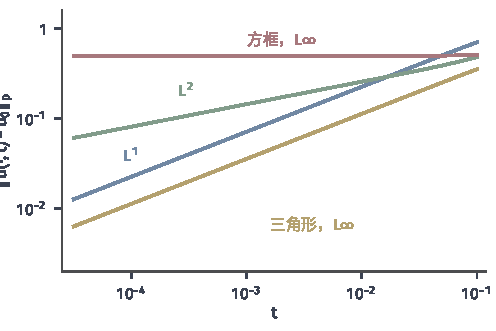
\includegraphics[width=84mm]{figures/06-differential-equations/02-partial-differential-equations/matplotlib/heat-recovery-norms/figure.pdf}
  \caption{解到初值的距离随$t$的变化，双对数坐标。方框初值$\mathbb{I}_{[-1/2,1/2]}$的$L^1$（蓝）、$L^2$（绿）、$L^\infty$（红）距离；连续三角形$\max\{1-\lvert x\rvert,0\}$的$L^\infty$距离（黄）。}
  \label{fig:heat-recovery-norms}
\end{BookInlineFigure}

\paragraph{连续点的恢复}
一般的初值只要在一点连续，解就在这一点取回初值，这是局部的结论，不需要整体的有界性。

\begin{theorem}[连续点的恢复]
\label{thm:heat-pointwise-recovery}
设$u_0$可测且满足式~\eqref{eq:heat-integrability}，在$\bm{x}_0$处连续。则
\begin{equation}
 \lim_{(\bm{x},t)\to(\bm{x}_0,0^+)}u(\bm{x},t)=u_0(\bm{x}_0) .
 \label{eq:heat-pointwise-recovery}
\end{equation}
\end{theorem}

\begin{proof}
仍利用$G$的积分为$1$，写成
\[
 u(\bm{x},t)-u_0(\bm{x}_0)=\int G(\bm{x}-\bm{y},t)\bigl(u_0(\bm{y})-u_0(\bm{x}_0)\bigr)\,\mathrm{d}\bm{y} .
\]
任取$\varepsilon>0$，取$\delta>0$使$\lvert\bm{y}-\bm{x}_0\rvert<\delta$时$\lvert u_0(\bm{y})-u_0(\bm{x}_0)\rvert<\varepsilon$。只考虑$\lvert\bm{x}-\bm{x}_0\rvert<\delta/2$。近处$\lvert\bm{y}-\bm{x}_0\rvert<\delta$的积分不超过$\varepsilon$。

在远处$\lvert\bm{y}-\bm{x}_0\rvert\geq\delta$，有$\lvert\bm{x}-\bm{y}\rvert\geq\delta/2$，并且$\lvert\bm{x}-\bm{y}\rvert$不小于$\lvert\bm{y}-\bm{x}_0\rvert/2$。

把指数平分成两半，一半用第一个下界，另一半用第二个下界：
\[
 \mathrm{e}^{-\lvert\bm{x}-\bm{y}\rvert^2/(4t)}\leq\mathrm{e}^{-\delta^2/(32t)}\,\mathrm{e}^{-\lvert\bm{y}-\bm{x}_0\rvert^2/(32t)} .
\]
限制$t\leq T/16$，并利用
\[
 \lvert\bm{y}-\bm{x}_0\rvert^2\geq\frac12\lvert\bm{y}\rvert^2-\lvert\bm{x}_0\rvert^2 ,
\]
第二个因子满足
\[
 \mathrm{e}^{-\lvert\bm{y}-\bm{x}_0\rvert^2/(32t)}\leq\mathrm{e}^{\lvert\bm{x}_0\rvert^2/(2T)}\,\mathrm{e}^{-\lvert\bm{y}\rvert^2/(4T)} .
\]

于是含$u_0(\bm{y})$的远处积分不超过
\[
 (4\pi t)^{-d/2}\,\mathrm{e}^{-\delta^2/(32t)}\,\mathrm{e}^{\lvert\bm{x}_0\rvert^2/(2T)}\int\lvert u_0(\bm{y})\rvert\,\mathrm{e}^{-\lvert\bm{y}\rvert^2/(4T)}\,\mathrm{d}\bm{y} .
\]
指数因子比$t^{-d/2}$衰减得快，所以这一项在$t\to0^+$时趋于零。

含常数$u_0(\bm{x}_0)$的远处积分不超过
\[
 \lvert u_0(\bm{x}_0)\rvert\int_{\lvert\bm{z}\rvert\geq\delta/2}G(\bm{z},t)\,\mathrm{d}\bm{z} ,
\]
由式~\eqref{eq:heat-tail}也趋于零。
\end{proof}

\paragraph{$L^\infty$的缺口}
能不能把三个定理合起来，说任意有界初值都一致恢复？不能。逐点恢复对每一点各用各的$\delta$，一致恢复要求同一个$\delta$对所有点有效，有界性也不能代替它。

取$d=1$、$u_0=\operatorname{sign}(x)$，解是$u=\operatorname{erf}(x/(2\sqrt{t}))$。对每个$x\neq0$它趋于$u_0(x)$，定理~\ref{thm:heat-pointwise-recovery}成立。但$u(0,t)=0$，$u$连续，在$0$右侧任意近处$u_0=1$而$u$接近$0$，所以对每个$t>0$，
\[
 \lVert u(\cdot,t)-u_0\rVert_\infty=1 .
\]

连续也不够。取$u_0=\sin(x^2)$，它有界连续但不一致连续。例~\ref{ex:heat-gaussian-growth}的Gauss积分对$a=\mathrm{i}$同样成立，其虚部就是解：
\[
 u(x,t)=\operatorname{Im}\Bigl[(1-4\mathrm{i}t)^{-1/2}\exp\Bigl(\frac{\mathrm{i}x^2}{1-4\mathrm{i}t}\Bigr)\Bigr] .
\]
取模得到包络$(1+16t^2)^{-1/4}\exp(-4x^2t/(1+16t^2))$，它在$\lvert x\rvert\to\infty$时趋于零。而$\sin(x^2)$在任意远处都取到$1$，所以对每个$t>0$，一致距离至少是$1$。图~\ref{fig:heat-sup-failure}画出了这两个例子。局部频率越高的地方被抹平得越快，每个$t>0$都有一片“已经抹平”的远场，它和初值相差一个固定的量。

\begin{BookInlineFigure}
  \centering
  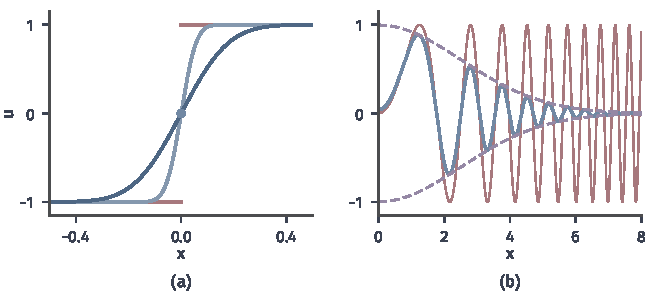
\includegraphics[width=112mm]{figures/06-differential-equations/02-partial-differential-equations/matplotlib/heat-sup-failure/figure.pdf}
  \caption{有界初值的一致恢复可能失败。(a)$u_0=\operatorname{sign}(x)$（红）与$t=0.001,0.01$的解（蓝色由浅到深），解在原点恒为零（蓝点）。(b)$u_0=\sin(x^2)$（红，细线）、$t=0.02$的解（蓝）与其包络（紫色虚线）。}
  \label{fig:heat-sup-failure}
\end{BookInlineFigure}

表~\ref{tab:heat-recovery}汇总了本节的结论。

\begin{BookInlineTable}
  \centering
  \caption{全空间热传播的初值恢复。}
  \label{tab:heat-recovery}
  \begin{tabular}{lll}
    \toprule
    初值 & 恢复方式 & 依据\\
    \midrule
    有界一致连续（含$C_0$） & 一致收敛 & 定理~\ref{thm:heat-uniform-recovery}\\
    $L^p$，$1\leq p<\infty$ & $L^p$收敛 & 定理~\ref{thm:heat-lp-recovery}\\
    满足式~\eqref{eq:heat-integrability} & 连续点处逐点收敛 & 定理~\ref{thm:heat-pointwise-recovery}\\
    一般$L^\infty$ & 一致收敛可能失败 & $\operatorname{sign}(x)$，$\sin(x^2)$\\
    \bottomrule
  \end{tabular}
\end{BookInlineTable}
